\documentclass[11pt, oneside]{report}  %can try book instead 	% use "amsart" instead of "article" for AMSLaTeX format
\usepackage[margin = 0.7in, bmargin = 1.1in, tmargin = 0.9in]{geometry}                		% See geometry.pdf to learn the layout options. There are lots.
\geometry{a4paper}                   		% ... or a4paper or a5paper or ... 
%\geometry{landscape}                		% Activate for rotated page geometry
\usepackage[parfill]{parskip}    		% Activate to begin paragraphs with an empty line rather than an indent
\usepackage{graphicx}				% Use pdf, png, jpg, or eps§ with pdflatex; use eps in DVI mode
								% TeX will automatically convert eps --> pdf in pdflatex		
\usepackage{amssymb}
\usepackage{amsmath}
\usepackage{amsmath,mathtools}
\usepackage{array}
\usepackage{tabu}
\usepackage{bm}
\usepackage{wrapfig}
\usepackage{multirow}
\usepackage{physics}
\usepackage{hyperref}
\usepackage{listings}
\usepackage[utf8]{inputenc}
\usepackage[T1]{fontenc}
\usepackage{lmodern}
%\usepackage{graphicx} %already declared above
\usepackage{caption}
\usepackage{float}
\usepackage{floatrow}
\usepackage{subfig}
\usepackage{multicol}
\usepackage{xcolor}
\usepackage{pagecolor}
\usepackage{lipsum}  
\usepackage{mdframed}
\usepackage{verbatim}
\usepackage{slashed}
%\usepackage[compat=1.1.0]{tikz-feynman}
%\usepackage{animate}


\newcommand{\G}{\mathcal{G}}
\newcommand{\D}{\mathcal{D}}
\newcommand{\E}{\mathcal{E}}
\renewcommand{\S}{\mathcal{S}}
\newcommand{\M}{\mathcal{M}}
\newcommand{\K}{\mathcal{K}}
\renewcommand{\L}{\mathcal{L}}
\newcommand{\R}{\mathcal{R}}
\renewcommand{\P}{\mathcal{P}}
\newcommand{\vp}{\varphi}
\newcommand{\T}{\mathcal{T}}
\newcommand{\A}{\mathcal{A}}
\newcommand{\bs}{\boldsymbol}
\newcommand{\rspace}{\mathbb{R}}
\newcommand{\dd}{\mathrm{d}}


\definecolor{purple}{RGB}{38,0,75}
\pagecolor{white}
\color{black}

%SetFonts

%SetFonts
\usepackage{subfiles} % Best loaded last in the preamble

\numberwithin{equation}{section}
\pagenumbering{gobble}
\title{Third Term Report}
\author{Robin Croft}
%\date{}	
\begin{document}





%\newpage
%\pagenumbering{arabic}


\section{Introduction}
general gr shit?
mention einstein derivation (hilbert derivation a potentially earlier but vacuum), karl schwarzshild ( ironicaly meaning black shield), then low mass limit, photon deflection and mercury perihelion around sun. mention cosmology, gravitational waves, more black holes, minkowski. more compact objects. 

\section{Introduction to Compact Objects and Boson Stars}
The first non-trivial solution to Einstein's equation found was that of the spherically symmetric, static and asymptotically flat vacuum spacetime by Karl Schwarzschild in 1915. The solution was designed to be used outside a spherically symmetric, non-spinning, body of mass; however it turned out to provide use in describing black holes. This metric was then modified by Tolman, Oppenheimer and Volkov in 1939 to describe the non-vacuum case of a constant density neutron star. This turned out to give an unphysical estimate of $0.7 M_\odot$ for the upper limit of neutron star mass due to the equation of state. 

The study of compact exotic objects can be traced back to John Wheeler who investigated Geons in 1955 for their potential similarity to elementary particles. Geons are gravito-electromagnetic objects with the name arising from "gravitational electromagnetic entity". In 1968 David Kaup published [] describing what he called "Klein-Gordon Geons", nowadays referred to as boson stars. Importantly, boson stars are a localised complex Klein-Gordon configuration, with the real counterparts being unstable. Many variants such as (Spin 1) proca stars [], electromagnetically charged boson stars and many others have been studied. 

Interest in boson stars remains for many reasons. Given the recent discovery of the higgs boson, we know that scalar fields exist in nature and any gravitational wave signals created by compact objects could theoretically be detected with modern gravitational wave interferometers. Secondly, boson stars are a good candidate for dark matter haloes. Boson stars are also useful as a proxy to other compact objects in general relativity; there is a lot of freedom in the construction of different types of boson star and they can be fine tuned to model dense neutron stars for one example. The advantage this would have over simulating a real fluid is that the Klein Gordon equation is linear in the principal part meaning smooth data must always remain smooth; thus avoiding shocks and conserving particle numbers relatively well with less sophisticated numerical schemes. 

On a slightly different topic, collisions of boson stars could be a natural method to produce scalar hair around black holes which will be discussed later in more detail. 

\subsection{Conventions}
Throughout this thesis physical quantities will be expressed as a dimensionless ratio of the Planck length, time and mass $L_{pl}$, $T_{pl}$ and $M_{pl}$ respectively; consequently the constants $c$, $G$ and $\hbar$ evaluate numerically to $1$. As an example, Newtons equation of gravity would be recast like
\begin{equation}
F = \frac{G M m}{r^2} \rightarrow \left(\frac{F}{F_{pl}} \right)=\frac{\left(\frac{M}{M_{pl}} \right)\left(\frac{m}{M_{pl}} \right)  }{\left(\frac{r}{L_{pl}} \right)^2}
\end{equation}
where $F_{pl} = M_{pl}L_{pl}T_{pl}^{-2}$ is the Planck force.
$c=G=\hbar=1$, unless stated otherwise. The metric signature will always be $(-,+,+,+)$. 

Tensor fields will be denoted using bold font for
index free notation and normal font for the components.
The dot product between two vector fields will be written interchangeably as $\bs{A} \cdot \bs{B} \leftrightarrow {A}_\mu {B}^\mu$ for readability.
Additionally, $\nabla_\mu$ denotes the covariant derivative and $\partial_\mu$
is the partial derivative, both with respect to coordinate $x^\mu$.

When considering the ADM decomposition, as in [REF SECT], objects can be associated with both the $3+1$ dimensional manifold $\M$ or the $3$ dimensional hypersurface $\Sigma$. To differentiate here, standard Roman letters such as $R$ represent the object belonging to $\M$ and calligraphic letters such as $\mathcal{R}$ correspond to the projected object belonging to $\Sigma$. [MAYBE JUST REMOVE THIS BIT AND MAKE IT OBVIOUS IN THE ACTUAL 3+1 SECTION].

Finally, unless stated otherwise, Greek indices such
as $\{\alpha, \beta, ..., \mu, \nu, ...\}$ label four dimensional tensor components whereas late Latin indices such as $\{i, j, k, ...\}$ label
three dimensional tensor components and early Latin indices such as $\{a, b, ...\}$ label two dimensional ones. When the index range is unspecified and unimportant Greek letters will also be used.

make explicit th inner product, dot product, outer product (otimes) and wedge product (for forms, antisymm)






\section{Differential Geometry}
\subsection{Introduction to Geometry / Manifolds (maybe change this)}
\begin{figure}{} %can add positioning here
\centering
    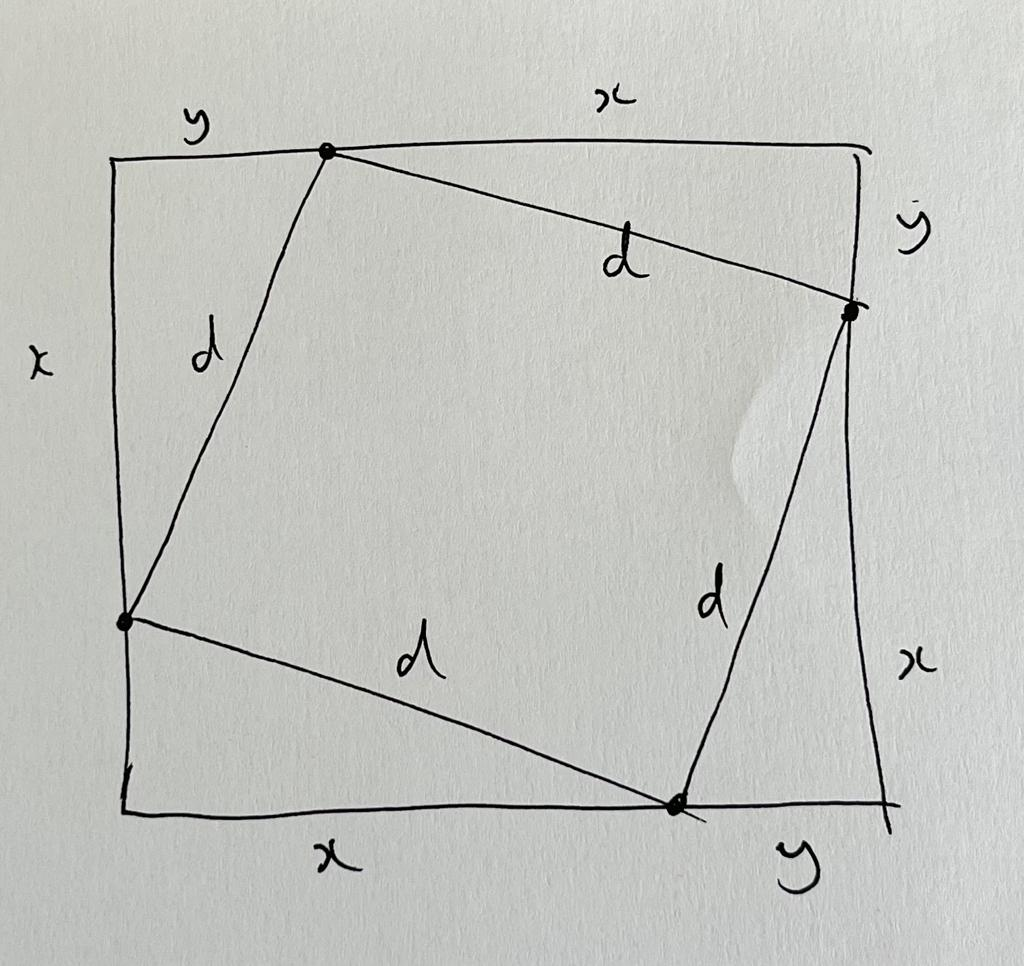
\includegraphics[width=0.35\textwidth]{../pics/pythag_proof.png}
    \caption{Diagram for proof of Pythagerous' theorem.}
    \label{fig:pythag_proof}
\end{figure}

From a young age, everyone has known Pythagerous' theorem $s^2 = x^2 + y^2$ for a right angled triangle with height $y$, width $x$ and hypotinuse length $s$. This can be shown very simply by looking at Fig.~\ref{fig:pythag_proof}. The area of the partially rotated square is obviously $s^2$, but we can also calculate it from the the area of the larger square $A_{sq}$ and subtracting four times the area of one of the triangles $A_{tr}$. Clearly $A_{sq} = (x+y)^2$ and $A_{tr} = \frac{1}{2}xy$, therefore 
\begin{equation}
s^2 = (x+y)^2-2xy = x^2 + y^2
\end{equation}
and we have proved Pythagerous' theorem. Using an infinitessimally small triangle, we can write $\dd s^2 = \dd x^2 + \dd y^2$ and this can be trivially extended to arbitrary dimensions like
\begin{equation}\label{eq:pythag_inf}
\dd s^2 = \dd x^2 + \dd y^2 + \dd z^2 + ...\,\,\,.
\end{equation}
The infinitessimal form of Pythagerous' theorem is very powerful as it lets us calculate the length of a generic curve by approximating the curve as a collection of infinitessimally small straight lines with length $\dd s$. So far we have assumed that space is flat meaning Eq.~(\ref{eq:pythag_inf}) is true for all points in space, this is an assumpion we will have to drop if we want to study gravity in the strong regime. In the next sections we will explore the generalisation of Pythagerous' equation to curved spaces and use it to measure curve lengths answell as volumes and areas.

Differential Geometry (DG) is the extension of calculus, linear algebra and multilinear algebra to general
geometries. Einstein’s Theory of Relativity is written using the language of DG as it is the natural
way to deal with curves, tensor calculus and differential tensor equations in curved spaces. For a basic
introduction to DG, we should start with a manifold $\M$ which is an $N$ dimensional space that locally looks
like $\rspace^N$, $N$ dimensional Euclidean space. This is important as at a point $p\in\M$ we can find infinitesimally
close neighbouring points $p + \delta p \in \M$. In the following sections we will explore how curves, functions, tensors and calculus are defined within DG.

\subsection{Functions, Curves and Tensors on Manifolds}
A real scalar function $f$ over $\M$ maps any point $p\in \M$ to a real number, this is denoted as
$f : p \rightarrow \rspace$. An important example of a set of scalar functions is the coordinate system $\phi$, $\phi : p \rightarrow \rspace^N$,
this is normally written $x^\mu$ where $\mu\in\{0,1,...,N-1\}$ is an index labelling the coordinate. The map $\phi$ is called a chart,
and unlike Euclidean space one chart may not be enough to cover the entire manifold; in this case a set
of compatible charts should be smoothly joined, collectively known as an atlas.

Now that functions have been discussed, the next simplest object we can discuss is a curve, or path, through $\M$. A curve $\Gamma$ is a set of smoothly connected points $p(\lambda)\in \M$ that smoothly depend on an input parameter $\lambda \in [\lambda_0,\lambda_1]$. This can be expressed in terms of coordinates as $x^\mu(\lambda)$ where $\phi:p(\lambda) \rightarrow x^\mu(\lambda)$. Differentiating a function $f$ along $\Gamma$ with respect to $\lambda$ gives
\begin{equation} \label{eq:dfdl}
\frac{\dd}{\dd \lambda}f(x^\mu(\lambda)) = \frac{\dd x^\nu}{\dd \lambda}\frac{\partial f(x^\mu)}{\partial x^\nu} = \frac{\dd x^\nu}{\dd \lambda}\partial_\nu f,
\end{equation}
where $\partial_\nu = {\partial}/{\partial x^\nu}$ and the Einstein summation convention was invoked, summing over all values of $\nu$. Equation~(\ref{eq:dfdl}) was derived independantly of the choice of $f$, therefore we can generally write
\begin{equation} \label{eq:ddl}
\frac{\dd}{\dd \lambda} = \frac{\dd x^\nu}{\dd \lambda}\partial_\nu.
\end{equation}
The operator $\dd/\dd \lambda $ can act on any function $f$ and return a new function $\tilde{f}$ over $\M$, formally this is written as $\dd/\dd \lambda (f) = \tilde{f}$ where $\tilde{f}:p\in\M\rightarrow \rspace$. We can also think of $\dd/\dd \lambda$ as a vector $\bs{X}$ with components $X^\mu=\dd x^\mu / \dd \lambda$ and basis vectors $\bs{e}_\mu:=\partial_\mu$ taken from Eq.~(\ref{eq:ddl}). The vector $\bs{X}$ can be written as $\bs{X} = X^\mu \bs{e}_\mu$ and can act on a general function $f$ over $\M$ as $\bs{X}(f) = X^\mu \bs{e}_\mu(f) = X^\mu \partial_\mu f$. 

Considering the set of all possible curves through a points $p\in\M$, the tangent vector components $\dd x^\mu / \dd \lambda$ span an $N$ dimensional space with basis $\bs{e}_\mu = \partial_\mu$; this space is called the tangent space and is denoted as $\T_p(\M)$. For the tangent space to be a vector space we need to define an inner product between two general vectors $\bs{X},\bs{Y} \in \T_p(\M)$, linear in it's arguments, like
\begin{equation}
(a\bs{X})\cdot(b \bs{Y}) = abX^\mu Y^\nu \bs{e}_\mu \cdot \bs{e}_\nu
\end{equation}
for any coefficients $a$ and $b$. In General Relativity it is helpful to define the dot product with the metric components $g_{\mu\nu}$ like $\bs{e}_\mu \cdot \bs{e}_\nu = g_{\mu\nu}$; alternatively 

\begin{equation}
\label{eq:metricXY}
\bs{X} \cdot \bs{Y} = X^\mu Y^\nu g_{\mu\nu}.\end{equation}

The next object to discuss is the co-vector which is defined as a map from vectors to real numbers; this is not the same as the dot product, and doesnt need one to exist [MAKE THIS BETTER]. Similarly to vectors, a co-vector $\bs{\omega}$ can be expressed as a sum of components $\omega_\mu$ and basis co-vectors $\bs{\theta}^\mu$ like $\bs{\omega} = \omega_\mu \bs{\theta}^\mu$. Contrary to vectors, co-vector components have downstairs indeces and the basis has upstairs indeces; this choice improves the readability of tensor equations when working with components. The power of co-vectors is that they map a vector to a real number like $\bs{\omega}:\bs{X} \rightarrow \rspace$ or $\bs{\omega}(\bs{X}) \rightarrow \rspace$. Vectors are equally able to map co-vectors to real numbers like $\bs{X}:\bs{\omega}\rightarrow\rspace$. Co-vectors are defined such that $\bs{\theta}^\mu : \bs{e}_\nu = \delta^\mu_\nu$ where $\delta^\mu_\nu$ are the components of the Kroneka delta equating to zero unless $\mu=\nu$ in which case they equal unity. The general operation of a co-vector $\bs{\omega}$ on a vector $\bs{X}$ is
\begin{equation}
\bs{\omega}: \bs{X} = \omega_\mu X^\nu \bs{\theta}^\mu:\bs{e}_\nu = \omega_\mu X^\nu \delta^\mu_\nu = \omega_\mu X^\mu \in \rspace.
\end{equation}
This map is linear and identical under reversing the order of operation; $\bs{\omega} : \bs{X} = \bs{X} : \bs{\omega}$. Similarly to vectors, the set of all possible co-vectors at a point $p\in\M$ span an N-dimensional space called the co-tangent space, written as $\T^*_p(\M)$.

Now that linear maps have been covered, we can generalise to multilinear maps and tensor fields. Consider a tensor field $\bs{T}$, this can be expressed in component form like 
\begin{equation}\bs{T} = T^{\alpha\beta, ...}_{\mu\nu,...} \bs{e}_\alpha\otimes\bs{e}_\beta \otimes... \otimes\bs{\theta}^\mu \otimes\bs{\theta}^\nu\otimes...
\end{equation}
for an arbitrary number of [MAKE THIS MAKE SNENSE]. A tensor field with $m$ co-vector bases and $n$ vector bases is called an $(m,n)$ tensor field, therefore vectors, co-vectors and scalars are $(1,0)$, $(0,1)$ and $(0,0)$ vectors respectively. Tensors can act as multilinear maps between tensor fields to other tensor fields. We have already seen how a vector and co-vector can map each other to a scalar, extending this we can use an $(0,2)$ tensor field $\bs{T}=T_{\mu\nu}\bs{\theta}^\mu\otimes\bs{\theta}^\nu$ to map two vector fields $\bs{X}$ and $\bs{Y}$ to a scalar like 
\begin{equation}
\bs{T}(\bs{X},\bs{Y}) = T_{\mu\nu}X^\alpha Y^\beta (\bs{\theta}^\mu:\bs{e}_\alpha)( \bs{\theta}^\nu:\bs{e}_\beta) = T_{\mu\nu}X^\mu Y^\nu.
\end{equation}
This equation is identical to Eq.~(\ref{eq:metricXY}) and we can see that the space-time metric is an $(0,2)$ tensor on our spacetime. As mentioned already, the multilinear map can output generic tensors, for example consider 
\begin{equation}
\bs{T}(\bs{X},\star) = T_{\mu\nu} X^\alpha (\bs{\theta}^\mu:\bs{e}_\alpha)\bs{\theta}^\nu = T_{\mu\nu}X^\mu \bs{\theta}^\nu,
\end{equation}
which uses the $(0,2)$ tensor $\bs{T}$ to map the vector $\bs{X}$ to a co-vector $\bs{W}$ with components $W_\mu = T_{\mu\nu}X^\mu$. One final example of a mapping is from a single tensor to a lower rank tensor, this is called contraction. To illustrate this, let's take a $(1,3)$ tensor $\bs{Z} = Z^\alpha_{\,\,\,\mu\nu\rho} \bs{e}_\alpha \otimes\bs{\theta}^\mu\otimes\bs{\theta}^\nu\otimes\bs{\theta}^\rho$. We can choose to use the basis vector $\bs{e}_\alpha$ to act on any of the three co-vector bases, choosing $\bs{\theta}^\mu$ this is
\begin{equation}
Z^\alpha_{\,\,\,\mu\nu\rho} (\bs{e}_\alpha : \bs{\theta}^\mu)\bs{\theta}^\nu\otimes\bs{\theta}^\rho = Z^\mu_{\,\,\,\mu\nu\rho}\bs{\theta}^\nu\otimes\bs{\theta}^\rho = \tilde{Z}_{\nu\rho}\bs{\theta}^\nu\otimes\bs{\theta}^\rho
\end{equation} 
where $\tilde{Z}_{\nu\rho} = Z^\mu_{\,\,\,\mu\nu\rho}$.

check faking field vs obect at a point p


\subsection{General Covariance / Coordinate transformations}

The power of tensor algebra and tensor calculus is that if a tensor equation can be written in one coordiante system then must hold (in abstact from) in any [NON-PATHOLOGICAL?] coordinate system. This is a consequence of the tensor transformation law and hence the saying "the definition of a tensor is an object that transforms like a tensor" [FIND QUOTE OR PUT THIS IN A BETTER PLACE?]. Looking back, we can write a generic vector field $\bs{X}$ as $X^\mu \bs{e}_\mu = X^\mu \partial_\mu$ and if we choose a coordinate transformation $x^\mu \rightarrow \tilde{x}^\mu$ then we see that in the transformed coordinate system the vector $\bs{X}$, written $\tilde{\bs{X}}$, becomes
\begin{align}
\tilde{\bs X} &= \tilde{X}^\mu\frac{\partial}{\partial \tilde{x}^\mu}, \\
              &= \tilde{X}^\mu\frac{\partial x^\nu}{\partial \tilde{x}^\mu}\frac{\partial}{\partial {x}^\nu}, \\
              &= X^\nu \frac{\partial}{\partial x^\nu}, \\
              &= \bs{X}, \
\end{align}
where $X^\nu = \tilde{X}^\mu\frac{\partial x^\nu}{\partial \tilde{x}^\mu}$ is required to make $\bs{X}=\tilde{\bs{X}}$. This says that the underlying geometric object (a vector in this case) is independant of the coordinates used to describe them; the tradeoff for this useful property is that the vectors components $X^\mu$ have to transform under the tensor transformation law, $\tilde{X}^\mu = \frac{\partial \tilde{x}^\mu}{\partial x^\nu} X^\nu$ [THIS IS TEH OTHER WAY ROUDN TO BEFORE]. Working from a co-vector $\omega$ we can write it as $\omega_\mu \bs{\theta}^\mu = \omega_\mu \dd x^\mu$ in component-basis form [REF THIS?] and the same coordinate transform gives
\begin{align}
\tilde{\bs{\omega}} &= \tilde{\omega}_\mu \dd \tilde{x}^\mu , \\
                    &= \tilde{\omega}_\mu \frac{\partial \tilde{x}^\mu}{\partial x^\nu}\dd {x}^\nu , \\
                    &= \omega_\nu \dd x^\nu,
\end{align}
where the co-vector components transform like $\omega_\nu= \tilde{\omega}_\mu \frac{\partial \tilde{x}^\mu}{\partial x^\nu}$, the opposite way to the vector components. These transformation laws ensure that a scalar field created from the product of a vector field and a co-vector field, like $\bs{\omega}:\bs{X}$, is a Lorentz scalar not transforming under coordinate transformations. This can be seen from
\begin{align}
\tilde{\bs \omega} : \tilde{\bs X} &= \tilde{X}^\mu \tilde{\omega}_\mu ,\\
                                   &= {X}^\nu \frac{\partial \tilde{x}^\mu}{\partial x^\nu}   \frac{\partial x^\rho}{\partial \tilde{x}^\mu}\omega_\rho, \\
                                   &=X^\nu \frac{\partial x^\rho}{\partial x^\nu} \omega_\rho , \\
                                   &=X^\nu \delta_\nu^{\,\,\rho} \omega_\rho , \\
                                   &=X^\nu\omega_\nu,\\
                                   &= \bs{\omega}:\bs{X}.
\end{align}
The general tensor transformation law comes from chaining multiple of the previous examples together [REWITE BETTER], for example
\begin{equation}
\tilde{T}^{\mu\nu,...}_{\,\,\,\,\,\rho\sigma,...} = T^{\alpha\beta,...}_{\,\,\,\,\,\gamma\delta,...}\left(
\frac{\partial \tilde{x}^\mu}{\partial x^\alpha}\frac{\partial \tilde{x}^\nu}{\partial x^\beta},...\times\frac{\partial x^\gamma}{\partial \tilde{x}^\rho}\frac{\partial x^\delta}{\partial \tilde{x}^\sigma},...\right).
\end{equation}


discuss coords, paths, vectoirs, forms, tensors, derivatives (lie, cov, partial ...), pullbacks (needed later), Riemann and stuff. see intro and appendix of smith kight. talk about forms? 0-form scalar, 1-form vector, 2-form antisymmetric 0,2 tensor ... exterior derivds and lie derivs?

use words lorentz invariant and covariant






\subsection{Differential Forms}
A differential $p$-form is an antisymetric $(0,p)$ tensor; the tensor components (e.g. $A_{\alpha\beta,...,\zeta}$) vanish if there is a repeating index, equal $1$ for an even permutation of indeces (like 1,2,3,...,N) and $-1$ for an odd permutation (such as 2,1,3,4,...,N). Note that a $0$-form is a function, a $1$-form is a co-vector and for an $N$-dimensional manifold the $N$-form is unique and the $p$-forms with $p>N$ vanish. 

When considering differential forms, the conventional covector basis is often changed from $\bs{\theta}^\mu$ to $\dd x^\mu$ which will lend itself nicely to integrating p-forms on manifolds later. This convention means we can write the metric as $\bs{g} = g_{\mu\nu} \dd x^\mu \otimes \dd x^\nu$; the same can be done for any tensor. Note that the metric cannot be a $2$-form as it is not a symmetric tensor, infact the metric is a symmetric tensor.


\subsection{Differentiation on Manifolds}
There are three types of derivative, all related to each other, that we care about on a manifold. [CHECK WHOLE PARAGRAPH] The simplest is the exterior derivative of a p-form, returning a $p+1$-form. For a $p$-form $\bs{A} = A_\mu \dd x^\mu$, the exterior derivative $\bs{F}=\dd\bs{A}$ is given by 
\begin{equation}
F_{\alpha\mu_a \mu_b , ... \mu_p} = \partial_{[ \alpha}A_{\mu_a \mu_b , ... \mu_p]},
\end{equation}
where the square brackets mean the antisymmetric [check as i might need epsilons here ]. This derivative guarentees to return a tensor without the need for a connection or metric on the manifold, unlike the partial derivative that we will see next. One common example of an exterior derivative is of a 1-form, say $\bs{A}$ giving 
\begin{equation}
(\dd A)_{\mu\nu} = \partial_\mu A_\nu - \partial_\nu A_\mu,
\end{equation}
and we will see soon, as with all exterior derivatives of forms, returns a tensor object.

The most common type of derivative is the coraviant derivative ($\nabla$), which reduces to the partial derivative ($\partial$) in flat space with cartesian coordinates. The purpose of the covariant derivative is to take a $(p,q)$ tensor $\bs{T}$ and return a $(p,q+1)$ tensor $\bs{\nabla T}$ which obeys the tensor transformatino law [REF]. For a scalar field $\varphi$ the partial derivative does obey the tensor transformation law for a co-vector, demonstraed here 
\begin{align}
\frac{\partial}{\partial \tilde{x}^\mu} \tilde{\varphi} &=\frac{\partial}{\partial \tilde{x}^\mu} {\varphi} ,\\
                                                        &=\frac{\partial x^\nu}{\partial\tilde{x}^\mu}\frac{\partial}{\partial {x}^\nu} {\varphi}
\end{align}
and therefore the components $\partial_\mu \varphi$ transform like a co-vector. Note the fact $\varphi=\tilde{\varphi}$ as a scalar remains unchanged in a coordinate transformation. Unfortunately, when taking the partial derivative of any other tensor we do not receive a new tensor; let's demonstrate this with a vector $X$.
\begin{align}
\frac{\partial}{\partial \tilde{x}^\mu} \tilde{X}^\alpha &= \frac{\partial}{\partial \tilde{x}^\mu}\left( \frac{\partial \tilde{x}^\alpha}{\partial x^\beta}{X}^\beta\right),\\
                                                         &= \frac{\partial x^\nu}{\partial \tilde{x}^\mu}\frac{\partial}{\partial \tilde{x}^\nu}\left( \frac{\partial \tilde{x}^\alpha}{\partial x^\beta}{X}^\beta\right),\\
                                                         &= \underbrace{\frac{\partial \tilde{x}^\alpha}{\partial x^\beta}\frac{\partial x^\nu}{\partial \tilde{x}^\mu}}_{\mathrm{Tensor}\,\,\rm{transformation}\,\,\rm{law}}\frac{\partial}{\partial \tilde{x}^\nu} {X}^\beta + {X}^\beta\frac{\partial x^\nu}{\partial \tilde{x}^\mu}\frac{\partial}{\partial \tilde{x}^\nu}\left( \frac{\partial \tilde{x}^\alpha}{\partial x^\beta}\right),\\
\end{align}
and only the term on the right obeys the tensor transformation law. Interestingly, if we take the exterior derivative from [REF dA] we see it transforms like 
\begin{align}
\frac{\partial}{\partial \tilde{x}^\mu}\tilde{A}_\nu - \frac{\partial}{\partial \tilde{x}^\nu} \tilde{A}_\mu &= 
\frac{\partial x^\rho}{\partial \tilde{x}^\mu}\frac{\partial}{\partial {x}^\rho}\left(\frac{\partial {x}^\sigma}{\partial\tilde{x}^\nu}A_\sigma\right) 
- \frac{\partial x^\sigma}{\partial \tilde{x}^\nu}\frac{\partial}{\partial {x}^\sigma}\left(\frac{\partial {x}^\rho}{\partial\tilde{x}^\mu}A_\rho\right) ,\\
&= \frac{\partial x^\rho}{\partial \tilde{x}^\mu}\frac{\partial {x}^\sigma}{\partial\tilde{x}^\nu}\left(\frac{\partial}{\partial {x}^\rho} A_\sigma - \frac{\partial}{\partial {x}^\sigma} A_\rho\right)
+ 
\frac{\partial x^\rho}{\partial \tilde{x}^\mu}\frac{\partial}{\partial {x}^\rho}\left(\frac{\partial {x}^\sigma}{\partial\tilde{x}^\nu}\right) A_\sigma
- \frac{\partial x^\sigma}{\partial \tilde{x}^\nu}\frac{\partial}{\partial {x}^\sigma}\left(\frac{\partial {x}^\rho}{\partial\tilde{x}^\mu}\right)A_\rho ,\\
&= \frac{\partial x^\rho}{\partial \tilde{x}^\mu}\frac{\partial {x}^\sigma}{\partial\tilde{x}^\nu}\left(\frac{\partial}{\partial {x}^\rho} A_\sigma - \frac{\partial}{\partial {x}^\sigma} A_\rho\right)
+ 
\left(  \frac{\partial^2 {x}^\rho}{\partial {x}^\mu\partial\tilde{x}^\nu} 
- \frac{\partial^2 {x}^\rho}{\partial\tilde{x}^\nu\partial\tilde{x}^\mu} \right)A_\rho ,\\
&= \frac{\partial x^\rho}{\partial \tilde{x}^\mu}\frac{\partial {x}^\sigma}{\partial\tilde{x}^\nu}\left(\frac{\partial}{\partial {x}^\rho} A_\sigma - \frac{\partial}{\partial {x}^\sigma} A_\rho\right),
\end{align}
and the tensor tranformation law is obeyed.

The final type of derivative we need is the Lie deivative, denoted $\L$. This maps a $(p,q)$ tensor to a $(p,q)$ tensor, acting as more of a directional derivative with respect to some vector $X$. It represents to rate of change of an object with respect to the inverse mapping of an infinitessimal diffeomorphism locally along vector $X^\mu$ [WRITE THIS BETTER]. Copy Lie reriv def here. A common Lie derivative is the derivative of a vector [DO] and the metric [DO] which leads to killings equaiton.

talk about linearity and liebnitz rule [check correct definitino]
derive covariant deriv and torsion free, metric compatibility.


\subsection{Integrating Forms on Manifolds}




\subsection{Length and Geodesics on Manifolds}
The natural entry point for studying calculus on manifolds it to revisit Pythagerous' theorem. For this we need a manifold $\M$ equipped with a metric $g$, written as $(\M,g)$ for short. [MAYBE NATURAL POINT IS LIE/OUTER DERIVS] The distance $\dd s$ between two infinitessimaly close points $p\in\M$ and $p+\delta p \in \M$, with coordinates $x^\mu$ and $x^\mu + \dd x^\mu$, is given by
\begin{equation}
\dd s^2 = g_{\mu\nu}\dd x^\mu \dd x^\nu,
\end{equation}
where $g_{\mu\nu}$ are the components of the metric tensor. This is the generalisation of Eq.~(\ref{eq:pythag_inf}) to curved space; noteably the line element can now have smoothly varying coefficients from $g_{\mu\nu}$ and cross terms such as $\dd x \dd y$. The special choice of $g_{\mu\nu} = \delta_{\mu\nu}$ gives us flat space, also called Euclidean space, where $\delta_{\mu\nu}=1$ if $\mu=\nu$ and vanishes otherwise. With the line elemend defines, we can immediately apply it to calculating the length of a general curve in curved space. Consider the curve $\Gamma$ consisting of a set of smoothly connected points $p(\lambda)\in\M$ smoothly parameterised by $\lambda$. We can calculate the length $\Delta s$ of the curve between $\lambda_1 \geq\lambda\geq\lambda_0$ by
\begin{align}
\dd s ^2 &= \frac{\partial x^\mu}{\partial \lambda}\frac{\partial x^\nu}{\partial \lambda}g_{\mu\nu}\dd \lambda^2,\\
\label{eq:Delta_s}\Delta s &= \int_{\lambda_0}^{\lambda_1}\sqrt{\left(\frac{\partial x^\mu}{\partial \lambda}\frac{\partial x^\nu}{\partial \lambda}g_{\mu\nu}\right)}\dd \lambda.
\end{align}
In the simplified case where $\lambda$ is one of the coordinates, say $\xi$, the length $\Delta s$ becomes,
\begin{align} \label{eq:coord_interval_length}
\Delta s &= \int_{\xi_0}^{\xi_1}\sqrt{g_{\xi\xi}}\dd \xi.
\end{align}

Now that lengths on manifolds have been discussed, we can approach volumes on manifolds. Take an $N$ dimensional manifold with metric $(\M,g)$ with coordinates $\{x_1,x_2,...,x_N\}$. 



line elements, integrals and derivatives?
Generalise this to algebraic metric rather than constant kroneka delta metric. Give exmaple in spherical polars. Maybe use this to calculate areas/lengths. Maybe insert picture of sphere. Insert proof that root det g is needed for volume elment from transforming a generic metric from one coord system to another? maybe need to invoke diff forms?


For a manifold equipped with metric $(\M,g)$ the curve with shortest distance between two points $p,q\in\M$ is called a geodesic. To find the geodesic joining $p$ and $q$ we need to use calculus of variation on the total length $\Delta s$ from Eq.~(\ref{eq:Delta_s}) of a general curve between two points. Given that the integrand $\L$ of Eq.~(\ref{eq:Delta_s}) is a function like $\L(x^\mu,\dot{x}^\mu)$, where the dot means differentiation by $\lambda$, we can use the Eular-Lagrange equation,
\begin{align}
\frac{\partial{\L}}{\partial x^\mu} - \frac{\dd}{\dd \lambda}\frac{\partial \L}{\partial \dot{x}^\mu} = 0
\end{align}
to give a differential equation with solution being a geodesic. Applyin the EL equation to the integrand of Eq.~(\ref{eq:Delta_s}) is algebraically messy, it is easier to square the integrand and start from $\L^2$ giving the same solution [EXPLAIN THIS BETTER]
\begin{align}
\frac{\partial{\L^2}}{\partial x^\alpha} &- \frac{\dd}{\dd \lambda}\frac{\partial \L^2}{\partial \dot{x}^\alpha} = 0, \\
\frac{\partial}{\partial x^\alpha} \left(g_{\mu\nu}\dot{x}^\mu\dot{x}^\nu\right) &- \frac{\dd}{\dd \lambda}\frac{\partial }{\partial \dot{x}^\alpha}\left(g_{\mu\nu}\dot{x}^\mu\dot{x}^\nu\right) = 0, \\
(\partial_\alpha g_{\mu\nu})\dot{x}^\mu\dot{x}^\nu &- 2\frac{\dd}{\dd \lambda}\left(g_{\alpha\nu}\dot{x}^\nu\right) = 0, \\
(\partial_\alpha g_{\mu\nu})\dot{x}^\mu\dot{x}^\nu &- 2\left(\dot{x}^\rho \partial_\rho \left(g_{\alpha\nu}\right)\dot{x}^\nu\right) - 2\ddot{x}^\nu g_{\alpha\nu} =0. 
\end{align}
Rearranging and multiplying by $g^{\alpha\beta}$ gives
\begin{align}
\ddot{x}^\beta &+ \frac{1}{2}g^{\alpha\beta}\left(\partial_{\mu}g_{\alpha\nu} +\partial_{\nu}g_{\alpha\mu} -\partial_{\alpha}g_{\mu\nu} \right)\dot{x}^\mu\dot{x}^\nu=0,\\
 \label{eq:geodesic}\ddot{x}^\beta &+ \Gamma^\beta_{\,\,\,\mu\nu}\dot{x}^\mu\dot{x}^\nu=0,
\end{align}
where $\Gamma^\beta_{\,\,\,\mu\nu}$ is the components of the connection-symbol from Eq.~(\ref{where ref?}). A trivial solution to Eq.~(\ref{eq:geodesic}) is in flat space using cartesian coordinates where $\Gamma^\beta_{\,\,\,\mu\nu}=0$ and therefore $\ddot{x}^\beta=0$ so $\dot{x}^\beta$ is a constant; this tells us the shortest distance between two points in flat space is a straight line. In other words, geodesics are straight lines in flat space.



\section{General Relativity}
General Relativity is

Einstein vacuum eqn, then add matter, maybe horizons and black holes stuff. check harvey/tong gr/bh notes for inspiration.

specific solutions like minkowski, gravitational waves, BH's, NS'

\subsection{Special Relativity}
gradient of metric go to zero, drops out SR?

1887 Michelson-Morley to find aether that light moves on. Instead found not true. laws of physics are the same in all frames. Assming these two things Einstein derived the Lorentz group.

\section{Stuff}
wheeler quote, matter tells space how to curve, adn space tells matter how to move.

GRChombo section?

einstein summation conventions? and upstiars/downstairs incedes in conventions

distinguish between tensors and tensor fields (especially in teh d/dlambda and X bit)

maybe work coordinate transformation into the text earlier with ther introduction of vectors? maybe split the long diff geom section (fucntions curves and tensors) into two sections, functions curves, coords trans, vectors part 1 then covectors, tensors and tensor transformation part 2, forms part 3 then differentiation then calculuas?

mention SR and the fact that GR is based on the equivalence principles (weak and strong?) somewhere .

maybe make SR as a solution to the Einstein eqation a different section to just SR.

\end{document}

